\documentclass{article}
\usepackage[utf8]{inputenc}
\usepackage{hyperref}

\title{Final Project Documentation}
\author{Ryan McHugh}
\date{April 2020}

\begin{document}

\maketitle

\setcounter{secnumdepth}{1}

\hypertarget{carberry-pi-documentation}{%
\subsection{Carberry Pi Documentation}\label{carberry-pi-documentation}}

// Logo

Carberry Pi

\begin{verbatim}

         11111111
        11   11   1
     111     11    1111
    111111111111111111111111
    1111001111111111110011111
      100001        100001
        00              00            
\end{verbatim}

\hypertarget{outline-of-this-document}{%
\subsection{Outline of this Document}\label{outline-of-this-document}}

\begin{enumerate}
\def\labelenumi{\arabic{enumi}.}
\item
  \protect\hyperlink{introduction}{Introduction}
\item
  \protect\hyperlink{hardware}{Hardware}
\item
  \protect\hyperlink{software}{Carberry Pi Software}

  3.1 \protect\hyperlink{dashboard}{Dashboard}

  3.2 \protect\hyperlink{diagnostics}{Diagnostics}

  3.3 \protect\hyperlink{configuration}{Configuration}

  3.4 \protect\hyperlink{displaying-engine-codes}{Displaying Engine
  Codes}

  3.5 \protect\hyperlink{architecture}{Architecture}
\item
  \protect\hyperlink{connecting-the-pieces}{Connecting the Pieces}
\item
  \protect\hyperlink{getting-up-and-running}{Getting Up and Running}
\end{enumerate}

\hypertarget{introduction}{%
\subsection{Introduction}\label{introduction}}

\begin{itemize}
\tightlist
\item
  \emph{Carberry Pi} is an automotive application of a mini-computer in
  the car. As the quintessential project for my undergraduate studies,
  this concept provides a deep-dive into an area of future interest.
\end{itemize}

\hypertarget{hardware}{%
\subsection{Hardware}\label{hardware}}

Carberry Pi requires a few tools of the trade.

~~~~Namely:

\begin{itemize}
\item
  Raspberry Pi (this project uses a Raspberry Pi 3 model B)
\item
  Professional Grade OBDII Cable
\item
  Raspberry Pi Touchscreen
\item
 \href{https://thepihut.com/products/mini-rtc-module-for-raspberry-pi}{DS3231 RTC IC}
  (Real Time Clock)
\end{itemize}

\hypertarget{carberry-pi-software}{%
\subsection{Carberry Pi Software}\label{carberry-pi-software}}

\hypertarget{dashboard}{%
\paragraph{Dashboard}\label{dashboard}}

\begin{figure}
\centering
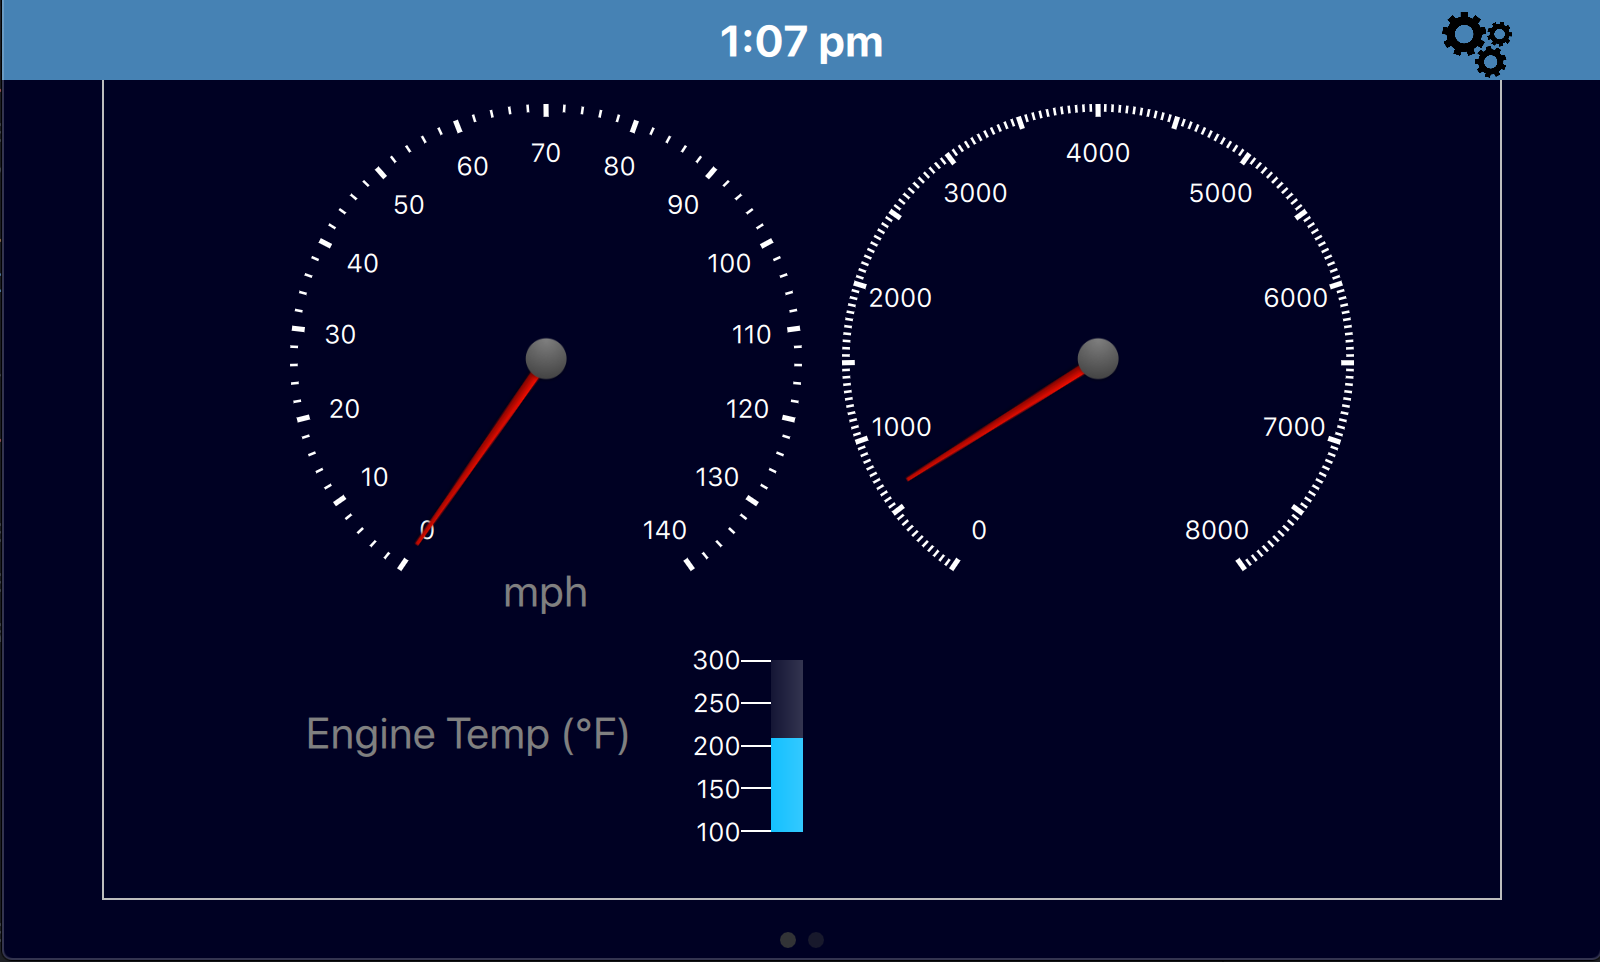
\includegraphics{./resources/dash.png}
\caption{Dashboard}
\end{figure}

\hypertarget{diagnostics}{%
\paragraph{Diagnostics}\label{diagnostics}}

\begin{figure}
\centering
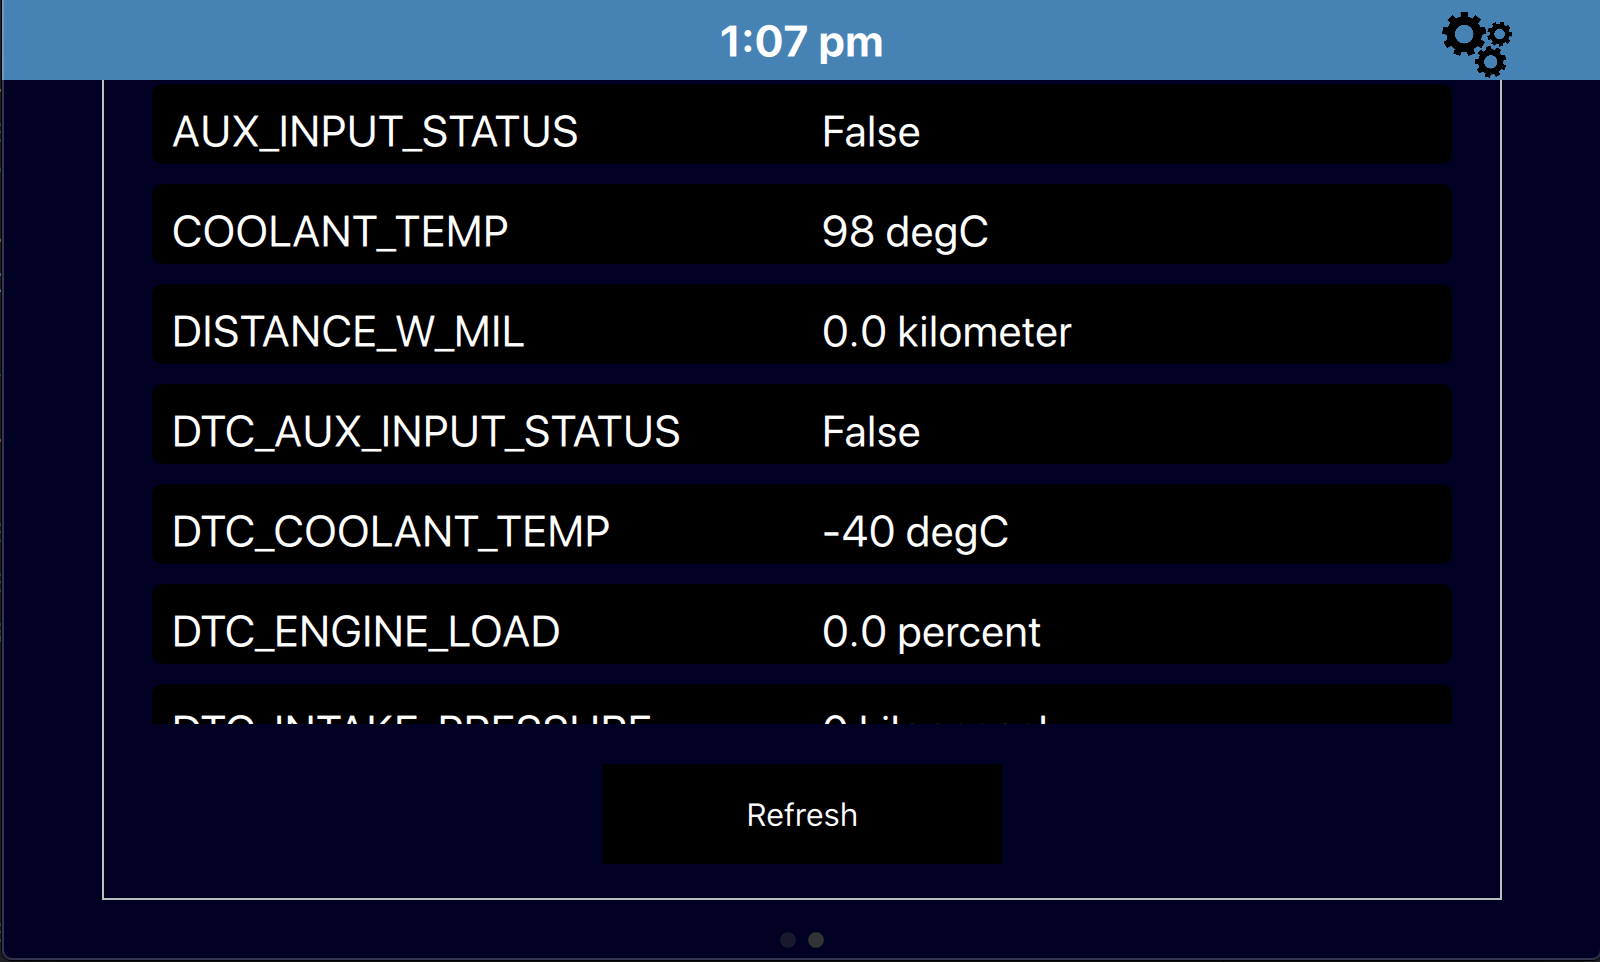
\includegraphics{./resources/diagnostics.png}
\caption{Diagnostics}
\end{figure}

\hypertarget{configuration}{%
\paragraph{Configuration}\label{configuration}}

\begin{figure}
\centering
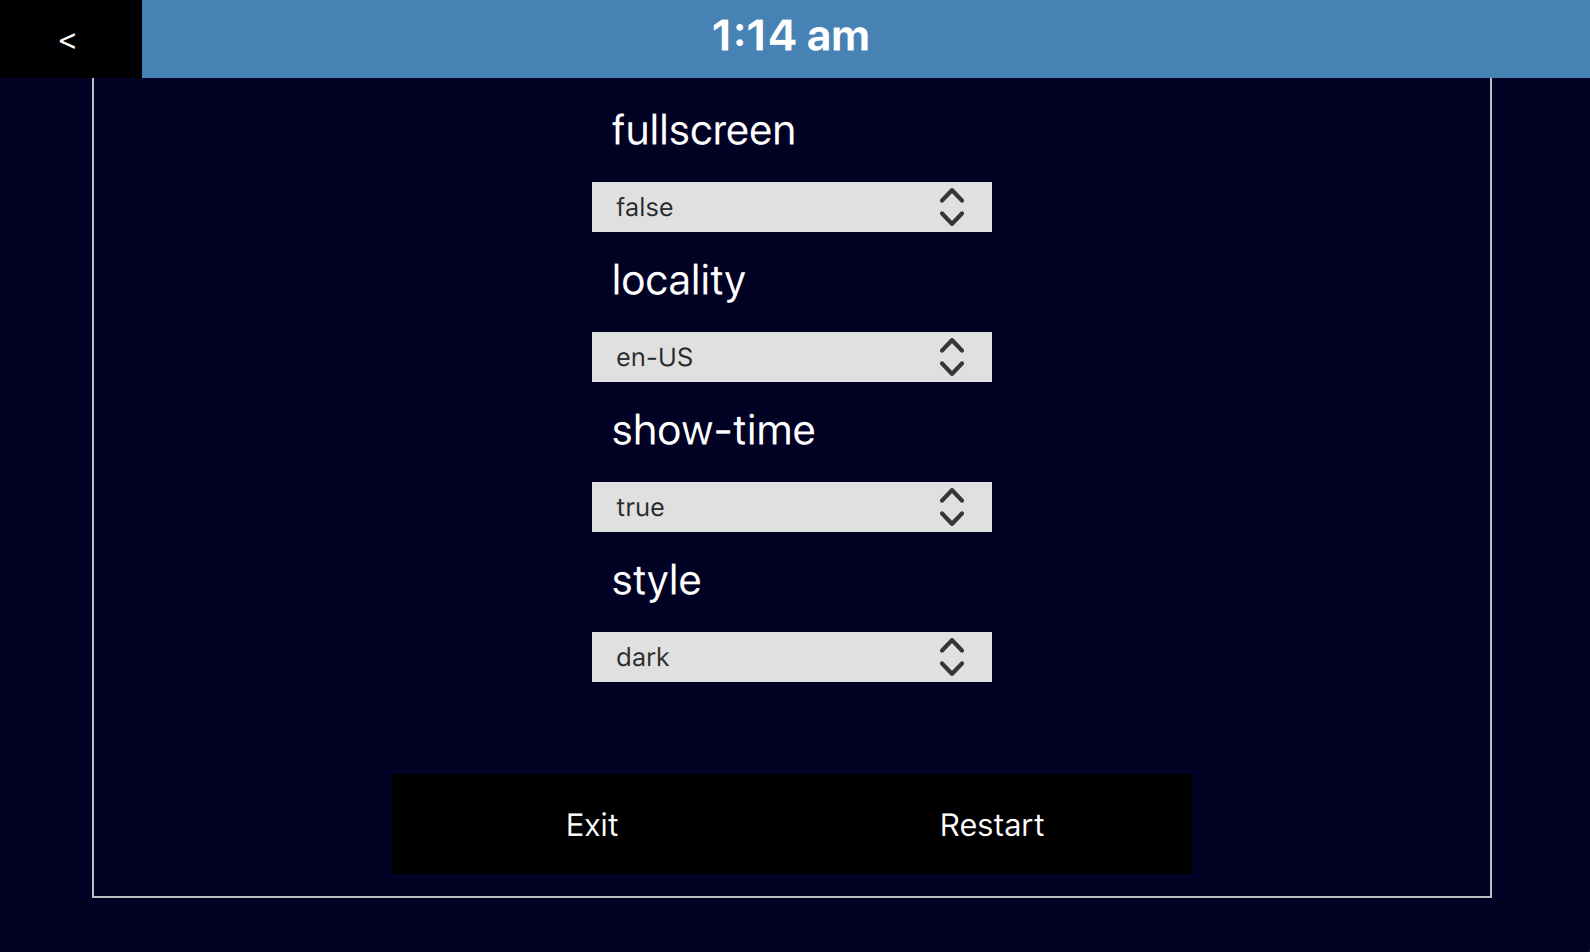
\includegraphics{./resources/configuration.png}
\caption{Configuration}
\end{figure}

\begin{itemize}
\tightlist
\item
  Currently a work-in-progress
\end{itemize}

\hypertarget{architecture}{%
\paragraph{Architecture}\label{architecture}}

\hypertarget{written-in__}{%
\subparagraph{Written in\_\_}\label{written-in__}}

\begin{itemize}
\item
  Backend: Python

  \begin{itemize}
  \tightlist
  \item
    Utilizes python-obd library for OBD information
  \end{itemize}
\item
  Frontend: PyQt (Qt-Quick Focused) \textbar{} Javascript
\end{itemize}

\hypertarget{interface-architecture}{%
\subparagraph{Interface Architecture}\label{interface-architecture}}

\begin{itemize}
\item
  Dynamic loading allows react-like module instantiation and destruction

  \begin{itemize}
  \item
    Each component is loaded into a \emph{view} as a separate entity
  \item
    These components can then be pushed/popped onto or from the
    main\emph{stackview}
  \item
    A separate script (javascript) manages the creation/destruction of
    the \emph{back} button
  \end{itemize}
\item
  Time

  \begin{itemize}
  \item
    The time is based on the RTC (Real Time Clock) of the Raspberry Pi
    itself.
  \item
    As such, changing the locality has no effect on the time value.
  \end{itemize}
\end{itemize}

\hypertarget{connecting-the-pieces}{%
\subsection{Connecting the Pieces}\label{connecting-the-pieces}}

// tutorial with picture layout of connecting each component

\hypertarget{getting-up-and-running}{%
\subsection{Getting Up and Running}\label{getting-up-and-running}}

\hypertarget{recommended-os-dietpi}{%
\paragraph{Recommended OS: DietPi}\label{recommended-os-dietpi}}

The \emph{DietPi} (debian-based) operating system distribution acts as a
lightweight desktop environment for running GUIs on the Pi.

Of Course, you may run this application on another operating system of
your choosing.

\textbf{Recommended DE: LXDE}

This project uses \emph{LXDE} as it is a lightweight desktop environment
that suits the limited hardware of the Rasperry Pi wonderfully.

** The \emph{autostart} functionality of the installation script
requires LXDE.

** The use of another desktop environment will require appending a
command that executes the \emph{start\_carberry.sh} script to the
startup file of the respective DE.





\end{document}
